\documentclass[11pt,letterpaper]{article}
\usepackage[margin=0.7in, includehead, includefoot, headheight=14pt, headsep=0.2in, footskip=0.35in]{geometry}
\usepackage[T1]{fontenc}
\usepackage[default]{sourcesanspro}
\usepackage{amsmath}
\usepackage{microtype}
\usepackage{xcolor}
\usepackage{tikz}
\usepackage{array}
\usepackage{tabularx}
\usepackage{booktabs}
\usepackage{enumitem}
\usepackage{titlesec}
\usepackage{needspace}
\usepackage{fancyhdr}

\pagestyle{fancy}
\fancyhf{}
\fancyhead[L]{Week 9 / Bouncing paths / Adult guide}
\fancyfoot[L]{Bellingham Math Circle / Week 9 / F09-FAC-v4}
\fancyfoot[R]{\thepage}
\renewcommand{\headrulewidth}{0pt}
\renewcommand{\footrulewidth}{0pt}

\setlength{\parindent}{0pt}
\setlength{\parskip}{4pt}
\raggedright
\setlist{nosep, leftmargin=1.2em, topsep=2pt}

\titleformat{\section}{\large\bfseries}{\thesection}{0.6em}{}
\titlespacing*{\section}{0pt}{9pt}{3pt}
\titleformat{\subsection}{\normalsize\bfseries}{}{0em}{}
\titlespacing*{\subsection}{0pt}{6pt}{2pt}

\definecolor{gridc}{gray}{0.72}
\colorlet{pathc}{black}
\newlength{\bpu}\setlength{\bpu}{0.14in}
% generated by check.py from the simulation; do not edit
\expandafter\def\csname bp-3-5-BL\endcsname{%
  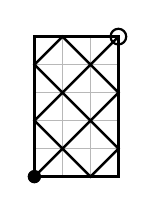
\begin{tikzpicture}[x=\bpu,y=\bpu,baseline=0pt]%
  \draw[gridc,line width=0.3pt] (0,0)--(0,5);%
  \draw[gridc,line width=0.3pt] (1,0)--(1,5);%
  \draw[gridc,line width=0.3pt] (2,0)--(2,5);%
  \draw[gridc,line width=0.3pt] (3,0)--(3,5);%
  \draw[gridc,line width=0.3pt] (0,0)--(3,0);%
  \draw[gridc,line width=0.3pt] (0,1)--(3,1);%
  \draw[gridc,line width=0.3pt] (0,2)--(3,2);%
  \draw[gridc,line width=0.3pt] (0,3)--(3,3);%
  \draw[gridc,line width=0.3pt] (0,4)--(3,4);%
  \draw[gridc,line width=0.3pt] (0,5)--(3,5);%
  \draw[line width=0.9pt] (0,0) rectangle (3,5);%
  \draw[pathc,line width=0.9pt] (0,0)--(1,1)--(2,2)--(3,3)--(2,4)--(1,5)--(0,4)--(1,3)--(2,2)--(3,1)--(2,0)--(1,1)--(0,2)--(1,3)--(2,4)--(3,5);%
  \fill (0,0) circle (0.24);%
  \draw[pathc,line width=0.8pt] (3,5) circle (0.28);%
  \end{tikzpicture}%
}
\expandafter\def\csname bp-3-5-BR\endcsname{%
  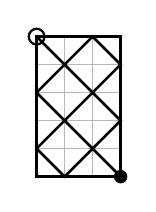
\begin{tikzpicture}[x=\bpu,y=\bpu,baseline=0pt]%
  \draw[gridc,line width=0.3pt] (0,0)--(0,5);%
  \draw[gridc,line width=0.3pt] (1,0)--(1,5);%
  \draw[gridc,line width=0.3pt] (2,0)--(2,5);%
  \draw[gridc,line width=0.3pt] (3,0)--(3,5);%
  \draw[gridc,line width=0.3pt] (0,0)--(3,0);%
  \draw[gridc,line width=0.3pt] (0,1)--(3,1);%
  \draw[gridc,line width=0.3pt] (0,2)--(3,2);%
  \draw[gridc,line width=0.3pt] (0,3)--(3,3);%
  \draw[gridc,line width=0.3pt] (0,4)--(3,4);%
  \draw[gridc,line width=0.3pt] (0,5)--(3,5);%
  \draw[line width=0.9pt] (0,0) rectangle (3,5);%
  \draw[pathc,line width=0.9pt] (3,0)--(2,1)--(1,2)--(0,3)--(1,4)--(2,5)--(3,4)--(2,3)--(1,2)--(0,1)--(1,0)--(2,1)--(3,2)--(2,3)--(1,4)--(0,5);%
  \fill (3,0) circle (0.24);%
  \draw[pathc,line width=0.8pt] (0,5) circle (0.28);%
  \end{tikzpicture}%
}
\expandafter\def\csname bp-2-2-BL\endcsname{%
  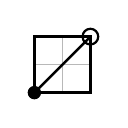
\begin{tikzpicture}[x=\bpu,y=\bpu,baseline=0pt]%
  \draw[gridc,line width=0.3pt] (0,0)--(0,2);%
  \draw[gridc,line width=0.3pt] (1,0)--(1,2);%
  \draw[gridc,line width=0.3pt] (2,0)--(2,2);%
  \draw[gridc,line width=0.3pt] (0,0)--(2,0);%
  \draw[gridc,line width=0.3pt] (0,1)--(2,1);%
  \draw[gridc,line width=0.3pt] (0,2)--(2,2);%
  \draw[line width=0.9pt] (0,0) rectangle (2,2);%
  \draw[pathc,line width=0.9pt] (0,0)--(1,1)--(2,2);%
  \fill (0,0) circle (0.24);%
  \draw[pathc,line width=0.8pt] (2,2) circle (0.28);%
  \end{tikzpicture}%
}
\expandafter\def\csname bp-1-3-BL\endcsname{%
  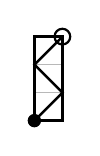
\begin{tikzpicture}[x=\bpu,y=\bpu,baseline=0pt]%
  \draw[gridc,line width=0.3pt] (0,0)--(0,3);%
  \draw[gridc,line width=0.3pt] (1,0)--(1,3);%
  \draw[gridc,line width=0.3pt] (0,0)--(1,0);%
  \draw[gridc,line width=0.3pt] (0,1)--(1,1);%
  \draw[gridc,line width=0.3pt] (0,2)--(1,2);%
  \draw[gridc,line width=0.3pt] (0,3)--(1,3);%
  \draw[line width=0.9pt] (0,0) rectangle (1,3);%
  \draw[pathc,line width=0.9pt] (0,0)--(1,1)--(0,2)--(1,3);%
  \fill (0,0) circle (0.24);%
  \draw[pathc,line width=0.8pt] (1,3) circle (0.28);%
  \end{tikzpicture}%
}
\expandafter\def\csname bp-2-1-BL\endcsname{%
  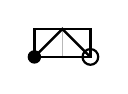
\begin{tikzpicture}[x=\bpu,y=\bpu,baseline=0pt]%
  \draw[gridc,line width=0.3pt] (0,0)--(0,1);%
  \draw[gridc,line width=0.3pt] (1,0)--(1,1);%
  \draw[gridc,line width=0.3pt] (2,0)--(2,1);%
  \draw[gridc,line width=0.3pt] (0,0)--(2,0);%
  \draw[gridc,line width=0.3pt] (0,1)--(2,1);%
  \draw[line width=0.9pt] (0,0) rectangle (2,1);%
  \draw[pathc,line width=0.9pt] (0,0)--(1,1)--(2,0);%
  \fill (0,0) circle (0.24);%
  \draw[pathc,line width=0.8pt] (2,0) circle (0.28);%
  \end{tikzpicture}%
}
\expandafter\def\csname bp-2-3-BL\endcsname{%
  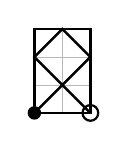
\begin{tikzpicture}[x=\bpu,y=\bpu,baseline=0pt]%
  \draw[gridc,line width=0.3pt] (0,0)--(0,3);%
  \draw[gridc,line width=0.3pt] (1,0)--(1,3);%
  \draw[gridc,line width=0.3pt] (2,0)--(2,3);%
  \draw[gridc,line width=0.3pt] (0,0)--(2,0);%
  \draw[gridc,line width=0.3pt] (0,1)--(2,1);%
  \draw[gridc,line width=0.3pt] (0,2)--(2,2);%
  \draw[gridc,line width=0.3pt] (0,3)--(2,3);%
  \draw[line width=0.9pt] (0,0) rectangle (2,3);%
  \draw[pathc,line width=0.9pt] (0,0)--(1,1)--(2,2)--(1,3)--(0,2)--(1,1)--(2,0);%
  \fill (0,0) circle (0.24);%
  \draw[pathc,line width=0.8pt] (2,0) circle (0.28);%
  \end{tikzpicture}%
}
\expandafter\def\csname bp-3-3-BL\endcsname{%
  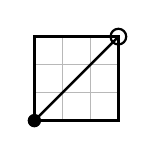
\begin{tikzpicture}[x=\bpu,y=\bpu,baseline=0pt]%
  \draw[gridc,line width=0.3pt] (0,0)--(0,3);%
  \draw[gridc,line width=0.3pt] (1,0)--(1,3);%
  \draw[gridc,line width=0.3pt] (2,0)--(2,3);%
  \draw[gridc,line width=0.3pt] (3,0)--(3,3);%
  \draw[gridc,line width=0.3pt] (0,0)--(3,0);%
  \draw[gridc,line width=0.3pt] (0,1)--(3,1);%
  \draw[gridc,line width=0.3pt] (0,2)--(3,2);%
  \draw[gridc,line width=0.3pt] (0,3)--(3,3);%
  \draw[line width=0.9pt] (0,0) rectangle (3,3);%
  \draw[pathc,line width=0.9pt] (0,0)--(1,1)--(2,2)--(3,3);%
  \fill (0,0) circle (0.24);%
  \draw[pathc,line width=0.8pt] (3,3) circle (0.28);%
  \end{tikzpicture}%
}
\expandafter\def\csname bp-3-2-BL\endcsname{%
  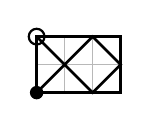
\begin{tikzpicture}[x=\bpu,y=\bpu,baseline=0pt]%
  \draw[gridc,line width=0.3pt] (0,0)--(0,2);%
  \draw[gridc,line width=0.3pt] (1,0)--(1,2);%
  \draw[gridc,line width=0.3pt] (2,0)--(2,2);%
  \draw[gridc,line width=0.3pt] (3,0)--(3,2);%
  \draw[gridc,line width=0.3pt] (0,0)--(3,0);%
  \draw[gridc,line width=0.3pt] (0,1)--(3,1);%
  \draw[gridc,line width=0.3pt] (0,2)--(3,2);%
  \draw[line width=0.9pt] (0,0) rectangle (3,2);%
  \draw[pathc,line width=0.9pt] (0,0)--(1,1)--(2,2)--(3,1)--(2,0)--(1,1)--(0,2);%
  \fill (0,0) circle (0.24);%
  \draw[pathc,line width=0.8pt] (0,2) circle (0.28);%
  \end{tikzpicture}%
}
\expandafter\def\csname bp-1-4-BL\endcsname{%
  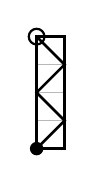
\begin{tikzpicture}[x=\bpu,y=\bpu,baseline=0pt]%
  \draw[gridc,line width=0.3pt] (0,0)--(0,4);%
  \draw[gridc,line width=0.3pt] (1,0)--(1,4);%
  \draw[gridc,line width=0.3pt] (0,0)--(1,0);%
  \draw[gridc,line width=0.3pt] (0,1)--(1,1);%
  \draw[gridc,line width=0.3pt] (0,2)--(1,2);%
  \draw[gridc,line width=0.3pt] (0,3)--(1,3);%
  \draw[gridc,line width=0.3pt] (0,4)--(1,4);%
  \draw[line width=0.9pt] (0,0) rectangle (1,4);%
  \draw[pathc,line width=0.9pt] (0,0)--(1,1)--(0,2)--(1,3)--(0,4);%
  \fill (0,0) circle (0.24);%
  \draw[pathc,line width=0.8pt] (0,4) circle (0.28);%
  \end{tikzpicture}%
}
\expandafter\def\csname bp-1-5-BL\endcsname{%
  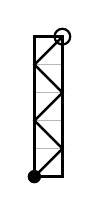
\begin{tikzpicture}[x=\bpu,y=\bpu,baseline=0pt]%
  \draw[gridc,line width=0.3pt] (0,0)--(0,5);%
  \draw[gridc,line width=0.3pt] (1,0)--(1,5);%
  \draw[gridc,line width=0.3pt] (0,0)--(1,0);%
  \draw[gridc,line width=0.3pt] (0,1)--(1,1);%
  \draw[gridc,line width=0.3pt] (0,2)--(1,2);%
  \draw[gridc,line width=0.3pt] (0,3)--(1,3);%
  \draw[gridc,line width=0.3pt] (0,4)--(1,4);%
  \draw[gridc,line width=0.3pt] (0,5)--(1,5);%
  \draw[line width=0.9pt] (0,0) rectangle (1,5);%
  \draw[pathc,line width=0.9pt] (0,0)--(1,1)--(0,2)--(1,3)--(0,4)--(1,5);%
  \fill (0,0) circle (0.24);%
  \draw[pathc,line width=0.8pt] (1,5) circle (0.28);%
  \end{tikzpicture}%
}
\expandafter\def\csname bp-2-5-BL\endcsname{%
  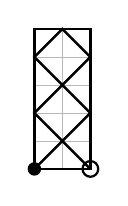
\begin{tikzpicture}[x=\bpu,y=\bpu,baseline=0pt]%
  \draw[gridc,line width=0.3pt] (0,0)--(0,5);%
  \draw[gridc,line width=0.3pt] (1,0)--(1,5);%
  \draw[gridc,line width=0.3pt] (2,0)--(2,5);%
  \draw[gridc,line width=0.3pt] (0,0)--(2,0);%
  \draw[gridc,line width=0.3pt] (0,1)--(2,1);%
  \draw[gridc,line width=0.3pt] (0,2)--(2,2);%
  \draw[gridc,line width=0.3pt] (0,3)--(2,3);%
  \draw[gridc,line width=0.3pt] (0,4)--(2,4);%
  \draw[gridc,line width=0.3pt] (0,5)--(2,5);%
  \draw[line width=0.9pt] (0,0) rectangle (2,5);%
  \draw[pathc,line width=0.9pt] (0,0)--(1,1)--(2,2)--(1,3)--(0,4)--(1,5)--(2,4)--(1,3)--(0,2)--(1,1)--(2,0);%
  \fill (0,0) circle (0.24);%
  \draw[pathc,line width=0.8pt] (2,0) circle (0.28);%
  \end{tikzpicture}%
}
\expandafter\def\csname bp-3-4-BL\endcsname{%
  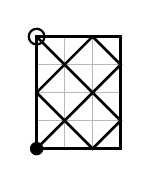
\begin{tikzpicture}[x=\bpu,y=\bpu,baseline=0pt]%
  \draw[gridc,line width=0.3pt] (0,0)--(0,4);%
  \draw[gridc,line width=0.3pt] (1,0)--(1,4);%
  \draw[gridc,line width=0.3pt] (2,0)--(2,4);%
  \draw[gridc,line width=0.3pt] (3,0)--(3,4);%
  \draw[gridc,line width=0.3pt] (0,0)--(3,0);%
  \draw[gridc,line width=0.3pt] (0,1)--(3,1);%
  \draw[gridc,line width=0.3pt] (0,2)--(3,2);%
  \draw[gridc,line width=0.3pt] (0,3)--(3,3);%
  \draw[gridc,line width=0.3pt] (0,4)--(3,4);%
  \draw[line width=0.9pt] (0,0) rectangle (3,4);%
  \draw[pathc,line width=0.9pt] (0,0)--(1,1)--(2,2)--(3,3)--(2,4)--(1,3)--(0,2)--(1,1)--(2,0)--(3,1)--(2,2)--(1,3)--(0,4);%
  \fill (0,0) circle (0.24);%
  \draw[pathc,line width=0.8pt] (0,4) circle (0.28);%
  \end{tikzpicture}%
}
\expandafter\def\csname bp-1-2-BL\endcsname{%
  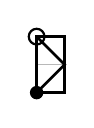
\begin{tikzpicture}[x=\bpu,y=\bpu,baseline=0pt]%
  \draw[gridc,line width=0.3pt] (0,0)--(0,2);%
  \draw[gridc,line width=0.3pt] (1,0)--(1,2);%
  \draw[gridc,line width=0.3pt] (0,0)--(1,0);%
  \draw[gridc,line width=0.3pt] (0,1)--(1,1);%
  \draw[gridc,line width=0.3pt] (0,2)--(1,2);%
  \draw[line width=0.9pt] (0,0) rectangle (1,2);%
  \draw[pathc,line width=0.9pt] (0,0)--(1,1)--(0,2);%
  \fill (0,0) circle (0.24);%
  \draw[pathc,line width=0.8pt] (0,2) circle (0.28);%
  \end{tikzpicture}%
}
\expandafter\def\csname bp-2-4-BL\endcsname{%
  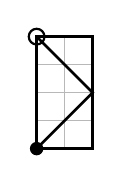
\begin{tikzpicture}[x=\bpu,y=\bpu,baseline=0pt]%
  \draw[gridc,line width=0.3pt] (0,0)--(0,4);%
  \draw[gridc,line width=0.3pt] (1,0)--(1,4);%
  \draw[gridc,line width=0.3pt] (2,0)--(2,4);%
  \draw[gridc,line width=0.3pt] (0,0)--(2,0);%
  \draw[gridc,line width=0.3pt] (0,1)--(2,1);%
  \draw[gridc,line width=0.3pt] (0,2)--(2,2);%
  \draw[gridc,line width=0.3pt] (0,3)--(2,3);%
  \draw[gridc,line width=0.3pt] (0,4)--(2,4);%
  \draw[line width=0.9pt] (0,0) rectangle (2,4);%
  \draw[pathc,line width=0.9pt] (0,0)--(1,1)--(2,2)--(1,3)--(0,4);%
  \fill (0,0) circle (0.24);%
  \draw[pathc,line width=0.8pt] (0,4) circle (0.28);%
  \end{tikzpicture}%
}
\expandafter\def\csname bp-3-6-BL\endcsname{%
  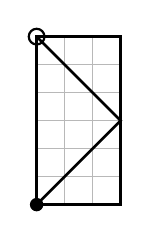
\begin{tikzpicture}[x=\bpu,y=\bpu,baseline=0pt]%
  \draw[gridc,line width=0.3pt] (0,0)--(0,6);%
  \draw[gridc,line width=0.3pt] (1,0)--(1,6);%
  \draw[gridc,line width=0.3pt] (2,0)--(2,6);%
  \draw[gridc,line width=0.3pt] (3,0)--(3,6);%
  \draw[gridc,line width=0.3pt] (0,0)--(3,0);%
  \draw[gridc,line width=0.3pt] (0,1)--(3,1);%
  \draw[gridc,line width=0.3pt] (0,2)--(3,2);%
  \draw[gridc,line width=0.3pt] (0,3)--(3,3);%
  \draw[gridc,line width=0.3pt] (0,4)--(3,4);%
  \draw[gridc,line width=0.3pt] (0,5)--(3,5);%
  \draw[gridc,line width=0.3pt] (0,6)--(3,6);%
  \draw[line width=0.9pt] (0,0) rectangle (3,6);%
  \draw[pathc,line width=0.9pt] (0,0)--(1,1)--(2,2)--(3,3)--(2,4)--(1,5)--(0,6);%
  \fill (0,0) circle (0.24);%
  \draw[pathc,line width=0.8pt] (0,6) circle (0.28);%
  \end{tikzpicture}%
}
\expandafter\def\csname bp-4-6-BL\endcsname{%
  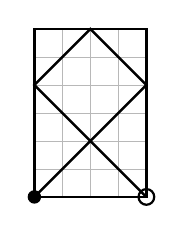
\begin{tikzpicture}[x=\bpu,y=\bpu,baseline=0pt]%
  \draw[gridc,line width=0.3pt] (0,0)--(0,6);%
  \draw[gridc,line width=0.3pt] (1,0)--(1,6);%
  \draw[gridc,line width=0.3pt] (2,0)--(2,6);%
  \draw[gridc,line width=0.3pt] (3,0)--(3,6);%
  \draw[gridc,line width=0.3pt] (4,0)--(4,6);%
  \draw[gridc,line width=0.3pt] (0,0)--(4,0);%
  \draw[gridc,line width=0.3pt] (0,1)--(4,1);%
  \draw[gridc,line width=0.3pt] (0,2)--(4,2);%
  \draw[gridc,line width=0.3pt] (0,3)--(4,3);%
  \draw[gridc,line width=0.3pt] (0,4)--(4,4);%
  \draw[gridc,line width=0.3pt] (0,5)--(4,5);%
  \draw[gridc,line width=0.3pt] (0,6)--(4,6);%
  \draw[line width=0.9pt] (0,0) rectangle (4,6);%
  \draw[pathc,line width=0.9pt] (0,0)--(1,1)--(2,2)--(3,3)--(4,4)--(3,5)--(2,6)--(1,5)--(0,4)--(1,3)--(2,2)--(3,1)--(4,0);%
  \fill (0,0) circle (0.24);%
  \draw[pathc,line width=0.8pt] (4,0) circle (0.28);%
  \end{tikzpicture}%
}
\expandafter\def\csname bp-1-1-BL\endcsname{%
  
\begin{tikzpicture}[x=\bpu,y=\bpu,baseline=0pt]%
  \draw[gridc,line width=0.3pt] (0,0)--(0,1);%
  \draw[gridc,line width=0.3pt] (1,0)--(1,1);%
  \draw[gridc,line width=0.3pt] (0,0)--(1,0);%
  \draw[gridc,line width=0.3pt] (0,1)--(1,1);%
  \draw[line width=0.9pt] (0,0) rectangle (1,1);%
  \draw[pathc,line width=0.9pt] (0,0)--(1,1);%
  \fill (0,0) circle (0.24);%
  \draw[pathc,line width=0.8pt] (1,1) circle (0.28);%
  \end{tikzpicture}%
}
\expandafter\def\csname bp-3-1-BL\endcsname{%
  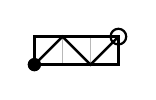
\begin{tikzpicture}[x=\bpu,y=\bpu,baseline=0pt]%
  \draw[gridc,line width=0.3pt] (0,0)--(0,1);%
  \draw[gridc,line width=0.3pt] (1,0)--(1,1);%
  \draw[gridc,line width=0.3pt] (2,0)--(2,1);%
  \draw[gridc,line width=0.3pt] (3,0)--(3,1);%
  \draw[gridc,line width=0.3pt] (0,0)--(3,0);%
  \draw[gridc,line width=0.3pt] (0,1)--(3,1);%
  \draw[line width=0.9pt] (0,0) rectangle (3,1);%
  \draw[pathc,line width=0.9pt] (0,0)--(1,1)--(2,0)--(3,1);%
  \fill (0,0) circle (0.24);%
  \draw[pathc,line width=0.8pt] (3,1) circle (0.28);%
  \end{tikzpicture}%
}

\newcommand{\bp}[3]{\csname bp-#1-#2-#3\endcsname}
% thumbnail with a two-line caption
\newcommand{\thumb}[5]{\begin{minipage}[b]{#4}\centering\bp{#1}{#2}{#3}\\[2pt]{\footnotesize #5}\end{minipage}}

% one problem block: label, core/further, page, what it is
\newcommand{\prob}[3]{\needspace{3\baselineskip}\par\smallskip\textbf{#1}\enspace\textit{#2}\enspace{\small(#3)}\par}
\newcommand{\what}{\textbf{Do:} }
\newcommand{\ans}{\textbf{Answer:} }
\newcommand{\hints}[3]{\textbf{Hints:} (1)~#1 (2)~#2\ifx&#3&\else{} (3)~#3\fi\par}
\newcommand{\core}{core}
\newcommand{\further}{further}

\begin{document}

{\LARGE\bfseries Bouncing paths: adult guide}\par
\smallskip
{\small K--1 packet F09-K-v4, grades 2--3 packet F09-M-v4, grades 4--5 packet F09-U-v4, all 8 pages. Section 4 has every answer, checked by \texttt{guide-src/check.py} against the boards on the final pages.}

\section{The idea of the week}

A ball rolls on a rectangle (the ``table'') drawn on squared paper. It starts at the bottom left corner, crosses each square slantwise from corner to corner, bounces off the walls, and stops when it lands in a corner of the table. For each table the children ask two questions: in which corner does the ball stop, and how many times does it bounce on the way?

Three facts carry the week. A bigger copy of a table (both sides doubled or tripled) behaves exactly like the small one: 2 by 3 and 4 by 6 both stop at the bottom right after 3 bounces. The ball never comes back to the corner it started from. And instead of bouncing the ball, you can flip a copy of the table over the wall and let the ball run straight on: the bouncing path becomes one straight line through copies of the table, and folding the copies up like a map turns the line back into the bouncing path.

Words on all three packets: ``a 7 by 3 table'' is 7 squares wide and 3 squares high. A bounce is each time the ball touches a wall; arriving in the final corner is not a bounce.

\medskip
\begin{tabularx}{\linewidth}{@{}>{\bfseries}l X@{}}
\toprule
Table & A good session \\
\midrule
K--1 & Every child walks the floor grid as the ball, and each pair traces at least six tables with a counter and a crayon, guessing the corner before each one. Good signs: a child guesses the 3 by 6 table from the 1 by 2 and 2 by 4; a child says ``it never comes back to the dot''.\\
2--3 & Careful paths with correct bounce counts on pages 1--2, then predictions on page 3 that use a smaller table (``8 by 12 is 2 by 3 made four times bigger''). Good signs: a reason why ``top right after 3 bounces'' is impossible; the complete list in Problem 6 with a reason.\\
4--5 & The chart filled far enough to see its patterns, a folding sheet made, and a rule for the corner and the bounces in terms of tables across and tables up. Good sign: a child's own explanation of why the ball never returns to its start.\\
\bottomrule
\end{tabularx}

\section{Materials and preparation}

Group: K--1 four children (two pairs); 2--3 four children (two pairs); 4--5 three children.

\smallskip
{\small
\begin{tabularx}{\linewidth}{@{}X l l l l@{}}
\toprule
Item & K--1 & 2--3 & 4--5 & Bring\\
\midrule
Counters, at most 3/4 inch across, two colours & 4 & 4 & 3 & 16\\
Rulers, 12 inch (30 cm) & 4 & 4 & 3 & 13\\
Pencils with erasers & 4 & 4 & 3 & 14\\
Crayons, chunky (box) & 2 & -- & -- & 3\\
Coloured pencils (pack) & 1 & 1 & 1 & 3\\
Black fine-tip permanent markers & 2 & 2 & 2 & 7\\
Scissors (child-safe at K--1) & 2 & 2 & 2 & 7\\
Clear tape (roll) & 1 & 1 & 1 & 3\\
Masking tape, about 60 ft (18 m), and a jump rope or 5 ft of string & 1 each & -- & -- & 1 each\\
Scrap paper to put under marker lines (sheets) & 3 & 3 & 3 & 10\\
\bottomrule
\end{tabularx}}

Counters: at K--1 each pair has one ``ball'' and one ``guess'' in different colours; at 2--3 and 4--5 each child has one to mark a guessed corner. Rulers, pencils: one per child. Crayons: a box per pair. Markers and scissors: one per pair (two at 4--5). Switching colour at every bounce makes bounces easy to count (number of colours minus one). The folding problems need a window or a lamp; a phone flashlight held under the paper also works.

\subsection{What to print}
US Letter, single-sided, at 100\% (``Actual size'', not ``Fit''). 111 student sheets in all.

\smallskip
{\small
\begin{tabularx}{\linewidth}{@{}l l l X@{}}
\toprule
Packet & Pages & Copies & How children use them\\
\midrule
K--1 & 1--7 & 3 each & One per pair plus a spare. Hand out one page at a time; partners share it and take turns, one table each.\\
K--1 & 8 & 6 & One per child plus 2 spares: each child cuts and folds their own squares.\\
2--3 & 1--8 & 5 & One packet per child plus a spare. Hand out a page at a time if the packet distracts.\\
2--3 & 5, 7 & +2 each & Spare game grid; spare folding sheets after a cutting mistake.\\
4--5 & 1--8 & 4 & One packet per child plus a spare.\\
4--5 & 3 & +6 & Two more blank tracing grids per child: the 36 tables of Problem 2 need 441 squares, one page has 224.\\
4--5 & 4 & +2 & Spare folding sheets.\\
\bottomrule
\end{tabularx}}

Each adult keeps the spare packet of their table and a copy of this guide. Nothing needs cutting in advance. Optional: cut out the three big squares on one K--1 page 8 for a child who finds cutting hard, since a ragged square folds badly.

\subsection{Floor grid for K--1 (set up before the children arrive, about 10 minutes)}
\begin{enumerate}
\item If the room has 12-inch (30 cm) floor tiles, use a block 3 tiles across and 5 tiles long and outline it with masking tape. The tile seams are the grid.
\item Otherwise tape a rectangle 4\textonehalf{} ft by 7\textonehalf{} ft (1.35 m by 2.25 m), mark every 18 inches (45 cm) along all four sides (an 18-inch strip of paper is a quick gauge), and run 2 tape lines the long way and 4 across. That gives 3 by 5 squares of 18 inches, using about 60 ft of tape.
\item Put the grid near the K--1 table. Make the outside walls stand out (double tape, or a second colour). Mark the two dots with a coloured tape X at both corners of one short end; that end is the ``bottom'' of the table. Leave the jump rope beside it.
\end{enumerate}

\textbf{How a child walks the path.} Stand on a dot, facing up the grid. Every step goes slantwise from a tape crossing to the opposite corner of the same square, never along a tape line. A big square may need a hop. When a step lands on an outside wall, everyone says ``bounce'' and counts. After a side wall, keep going up the grid but slant the other way; after the far end, keep slanting the same way but come back down the grid. Stop on landing in a corner of the big rectangle. Before each walk the others stand at the corner where they think the ball will stop.

\subsection{Test before the session (10 minutes, with the printed pages)}
\begin{enumerate}
\item Measure the squares: 3/4 inch on the K--1 pages, 1/2 inch on the others. Smaller squares mean the printer scaled the page; reprint at 100\%.
\item Put a counter on a corner of a K--1 square. It must not cover the next corner, 3/4 inch away.
\item Make one folding sheet yourself (2--3 page 7, top sheet). Draw the diagonal with the marker, cut out the 4 tables the line passes through as one piece, fold backward on the thick lines from the far end toward the dot table, and hold the stack against a window or lamp. The line must show through 4 layers. If it does not, press harder with the marker, use daylight, or shine a phone flashlight from behind. Keep your folded example for a stuck child.
\item Walk the floor grid from each dot. Both walks end at the far opposite corner after 6 bounces (picture in section 4).
\end{enumerate}

\section{The hour}

\begin{tabularx}{\linewidth}{@{}l X@{}}
\toprule
0:00--0:05 & Running around.\\
0:05--0:08 & Launch at the floor grid, everyone.\\
0:08--0:50 & Work at the three tables.\\
0:50--0:55 & Sharing question, everyone.\\
0:55--1:00 & Tidy up. Adults jot notes for section 6.\\
\bottomrule
\end{tabularx}

\subsection{Launch (organizer, 2--3 minutes)}
The children stand around the outside of the floor grid.
\begin{enumerate}
\item Stand on the left dot. Say: ``This tape is a pool table. The outside line is the wall. I'm the ball, and I start in this corner.''
\item Take one slanted step to the opposite corner of the first square. Say: ``The ball always goes slanted, across one square from corner to corner. Never along a line.''
\item Say: ``Who wants to be the ball?'' A K--1 child stands on the dot and takes three slanted steps, landing on the right-hand wall. Say: ``You hit the wall. Everybody say `bounce'.'' Point up the grid: ``The ball keeps going up the table, but now it slants back the other way.'' The child takes one step up and to the left. That step after the wall is the legal move everyone needs to see.
\item Say: ``The ball keeps going until it lands exactly in a corner of the table, and there it stops. Landing in the corner is not a bounce. Where will this ball stop? Don't say. The K--1 table will walk it and find out.''
\item Say: ``At your tables you'll do the same on paper with a counter or a pencil. Before each table, your partner guesses where the ball will stop.''
\end{enumerate}

\subsection{Pairs}
\begin{itemize}[leftmargin=2.9em, labelwidth=2.5em, labelsep=0.4em, align=left, itemsep=2pt]
\item[\textbf{K--1}] Two pairs, a kindergartner with a first grader if possible. For each table the guesser puts the guess counter on a corner; the mover moves the ball counter one square at a time from the dot and draws the path behind it with a crayon; both count bounces aloud. Swap after each table. Problem 1 is done by all four at the floor grid: one walks, three guess by standing at a corner.
\item[\textbf{2--3}] Two pairs. The predictor writes a corner and a bounce count under the table before the tracer starts; the tracer traces in pencil. Swap after each table. Problem 5 is a game inside each pair.
\item[\textbf{4--5}] A pair and a referee. The predictor commits (counter on a corner, bounce count written), the tracer traces, the referee checks every step and the count. Rotate after each problem. For the Problem 2 chart each child takes two widths (1--2, 3--4, 5--6), and each checks a neighbour's column.
\end{itemize}

\subsection{When attention runs out}
\begin{itemize}[leftmargin=2.9em, labelwidth=2.5em, labelsep=0.4em, align=left, itemsep=2pt]
\item[\textbf{K--1}] Back to the floor grid with the jump rope. Lay it across the grid to make a shorter table, or along it to make a narrower one. Children guess by standing on a corner, then one walks. From the left dot: rope 1 square up (3 by 1) far right, 2 bounces; 2 up (3 by 2) far left, 3; 3 up (3 by 3) far right, 0; 4 up (3 by 4) far left, 5. Rope the long way leaving 2 columns (2 by 5): near right, 5 bounces; leaving 1 column (1 by 5): far right, 4.
\item[\textbf{2--3}] Problem 5 as a stand-alone game, or ``stump the adult'': a child draws any table up to 12 by 12, the adult predicts corner and bounces without tracing, the children trace to check. They will want to know how the adult does it, which leads back to Problem 3.
\item[\textbf{4--5}] ``Stump the referee'': one child draws a table on a spare page 3 grid, the other two predict corner and bounces without tracing (a point for each), the referee traces to check. Rotate.
\end{itemize}

\subsection{Sharing question (all tables, 5 minutes)}
\textbf{``Did anyone find a table where the ball stops back at the dot where it started?''} Ask K--1 first (what they tried on page 7), then 2--3, then let a 4--5 child give a reason if there is one. Without a reason, ``we never found one'' is the honest status of the claim.

\section{Table by table}

Abbreviations for the older tables: TL top left, TR top right, BR bottom right; ``TR 6'' means it stops at the top right after 6 bounces. Slips to watch for at every table: counting the arrival in the corner as a bounce; stopping at a point on a wall that is not a corner of the table; stopping where the path crosses itself (the ball goes straight through its own path).

\subsection{K--1 (parent volunteer)}
\textbf{Core of the hour:} Problems 1--3. \textbf{For children who get further:} Problems 4--7. \textbf{If a child is struggling:} stay with the small tables (2 by 2, 1 by 3 and 2 by 1 on page 2; 1 by 2 on page 4), move the counter for them while they say ``bounce'' at each wall, and skip the 2 by 5, 3 by 4 and 4 by 6 tables and Problem 5.

\textbf{Things to say:} ``Slanted, corner to corner.'' ``Which wall did it hit? So which way now?'' ``Put your guess counter down first.'' ``Is the ball in a corner of the table? Then it stops.'' In the pictures below the dot is the start and the ring is where the ball stops.

\prob{Problem 1}{\core}{page 1, floor grid}
\what Each child walks once from each dot while the others guess; then each pair draws both walks on page 1.\\
\ans From the left dot: the far right corner, 6 bounces (15 steps). From the right dot: the far left corner, 6 bounces. The path crosses itself four times; the walker just keeps going.

\thumb{3}{5}{BL}{0.9in}{left dot}\hspace{0.3in}\thumb{3}{5}{BR}{0.9in}{right dot}

\hints{``Which way were you slanting before the wall? Keep going up the room and slant the other way.''}{Walk beside the child saying each step: ``slant, slant, bounce''.}{Put a counter or a shoe on the floor at each bounce so the drawing can be copied from the floor.}

\prob{Problem 2}{\core}{page 2}
\what Six tables: draw each path and show where the ball stops.\\
\ans\par\nopagebreak
\thumb{2}{2}{BL}{0.95in}{2 by 2\\top right, 0}\hfill
\thumb{1}{3}{BL}{0.95in}{1 by 3\\top right, 2}\hfill
\thumb{2}{1}{BL}{0.95in}{2 by 1\\bottom right, 1}\hfill
\thumb{2}{3}{BL}{0.95in}{2 by 3\\bottom right, 3}\hfill
\thumb{3}{3}{BL}{0.95in}{3 by 3\\top right, 0}\hfill
\thumb{3}{2}{BL}{0.95in}{3 by 2\\top left, 3}\par
\hints{``Put the ball counter on the dot. Which square does it cross first?''}{Move the counter one square at a time and stop at each wall: ``Which way now? Keep going up, and turn away from the wall.''}{Move the counter yourself while the child draws behind it.}

\prob{Problem 3}{\core}{page 3}
\what Count the bounces on four tables and write the number in the box.\\
\ans\par\nopagebreak
\thumb{1}{4}{BL}{0.95in}{1 by 4\\3 (top left)}\hfill
\thumb{1}{5}{BL}{0.95in}{1 by 5\\4 (top right)}\hfill
\thumb{2}{5}{BL}{0.95in}{2 by 5\\5 (bottom right)}\hfill
\thumb{3}{4}{BL}{0.95in}{3 by 4\\5 (top left)}\par
On the one-square-wide tables the ball touches a wall at every step except the last.\\
\hints{``Tap the wall with your finger each time the ball touches it, and count out loud.''}{Make a small mark on the wall at each bounce, or change crayon colour at each bounce, then count.}{``The corner at the end doesn't count. Did you count it?''}

\prob{Problem 4}{\further}{pages 4--5}
\what Draw the path and count the bounces on 1 by 2, 2 by 4, 3 by 6, then 2 by 3 and 4 by 6. Ask for a guess before the 3 by 6 and the 4 by 6.\\
\ans\par\nopagebreak
\thumb{1}{2}{BL}{0.95in}{1 by 2\\top left, 1}\hfill
\thumb{2}{4}{BL}{0.95in}{2 by 4\\top left, 1}\hfill
\thumb{3}{6}{BL}{0.95in}{3 by 6\\top left, 1}\hfill
\thumb{2}{3}{BL}{0.95in}{2 by 3\\bottom right, 3}\hfill
\thumb{4}{6}{BL}{0.95in}{4 by 6\\bottom right, 3}\par
A bigger copy of a table does exactly what the small one does.\\
\hints{``Which table on this page looks like a big version of the little one?''}{Put the 1 by 2 next to the 2 by 4: ``Same corner? Same number of bounces?''}{Trace the big one together with the counter.}

\prob{Problem 5}{\further}{page 6}
\what For each little picture, draw a table on one of the two grids so that the ball stops at the corner with the circle.\\
\ans Every table that fits the 3 by 3 grids. Top left: 1 by 2 or 3 by 2. Bottom right: 2 by 1 or 2 by 3. Top right: 1 by 1, 1 by 3, 2 by 2, 3 by 1 or 3 by 3.\\
\hints{``Look back at pages 2 to 4. Which tables stopped at the top left?''}{``Draw one and trace it. If it misses, use the other grid.''}{Top left: try one square wide and two tall. Bottom right: two wide and one tall. Top right: any square.}

\prob{Problem 6}{\further}{page 7}
\what Try to draw a table where the ball comes back to the dot and stops there.\\
\ans There is none. Children try several tables and each ends somewhere else; ``we tried lots and it never came back'' is a good K--1 answer. If a child says they found one, trace it again slowly together: usually the ball was stopped at a point that is not a corner of the table.\\
\hints{``Try a different shape on the next grid. Where did it end?''}{``Look at all the tables you did today. Did any come back to the dot?''}{A reason an older child can give: to come home the ball would have to come down its very first slanted step backwards, so somewhere it would have to turn right around. The ball only turns right around in a corner, and there it would already have stopped.}

\prob{Problem 7}{\further}{page 8}
\what With a ruler, draw a straight line from the dot to the far corner of each big square; cut the square out; fold on the dashed lines, folding the other parts back behind the dot part; hold it up to the light and draw the line you see on the small table beside it.\\
\ans The folded line is the ball's path. 2 by 2 square: the 1 by 2 path (top left, 1 bounce). 3 by 3 square: the 1 by 3 path (top right, 2 bounces). 4 by 4 square: the 2 by 4 path (top left, 1 bounce). These match the paths on pages 2 and 4.\\
\hints{Hold the ruler while the child draws with the marker.}{Fold backward and crease hard with a fingernail, dot side facing the child.}{Hold the folded square flat against the window.}

\subsection{Grades 2--3 (mathematician)}
\textbf{Core:} Problems 1--4. \textbf{Further:} 5--8. \textbf{If a child is struggling:} in Problem 1 do only 2 by 3, 3 by 2 and 1 by 4; in Problem 2 do the top row; skip Problem 3 and play the Problem 5 game with tables up to 4 by 4.

\prob{Problem 1}{\core}{page 1}
\ans 2 by 3 BR 3; 3 by 2 TL 3; 1 by 4 TL 3; 3 by 4 TL 5; 4 by 3 BR 5; 3 by 5 TR 6.\\
\hints{``Put your pencil on the dot. Which wall does it hit first, and where?''}{``At a side wall, which changes: going up or down, or going left or right?''}{``Make a tick on the wall at each bounce and count the ticks. The last corner gets no tick.''}

\prob{Problem 2}{\core}{page 2}
\ans 1 by 2, 2 by 4, 3 by 6: all TL 1. 1 by 3 and 2 by 6: TR 2. 4 by 6: BR 3 (it is 2 by 3 doubled, not a copy of 1 by 3).\\
\hints{``Which table on this page is the 1 by 2 table made bigger?''}{``Before you trace the 3 by 6, what do you expect?''}{Use the Problem 1 hints for the tracing itself.}

\prob{Problem 3}{\core}{page 3}
\what Predict, then trace. \ans 5 by 10: TL 1 (1 by 2 made five times bigger). 8 by 12: BR 3 (2 by 3 made four times bigger).\\
\hints{``Is this table a bigger copy of one you have traced? Which one?''}{``Look at 1 by 2, 2 by 4, 3 by 6 on page 2. What happened to the corner and the bounces?''}{``Divide both sides of 8 by 12 by the same number. What table do you get?''}

\prob{Problem 4}{\core}{page 4, grids 6 by 6}
\ans Every solution that fits. BR after 1 bounce: 2 by 1, 4 by 2, 6 by 3. TR after 4: 1 by 5, 5 by 1. TL after 7: 5 by 4 only. TR after 3: impossible.\\
\textbf{Why ``TR after 3'' is impossible, as a child can say it:} each bounce off a side wall switches the ball between going right and going left. It starts going right and arrives at a right-hand corner going right, so it bounced off the side walls an even number of times. In the same way it starts going up and arrives at the top going up, so it bounced off the top and bottom an even number of times. Even plus even is even, so a top right stop never has 3 bounces. (The children can check: every TR on pages 1--2 has 2 or 6.)\\
\hints{``Which tables on pages 1--2 stopped at the bottom right? Which bounced once?''}{For TR after 4: ``Try a table one square wide.'' For TL after 7: ``Try tables with a side of 4 or 5.''}{For TR after 3: ``List the bounce counts of all your top right tables. What do you notice?''}

\prob{Problem 5}{\further}{page 5, game}
\what One child draws a table up to 6 by 6, the partner predicts corner and bounces and then traces; 1 point for the corner, 1 for the bounces; three tables each. Check any table up to 6 by 6 in the chart in the 4--5 section below. If the grid fills, use a spare page 5.\\
\hints{``Is this table a bigger copy of a smaller one?''}{``Which of your traced tables is it most like?''}{}

\prob{Problem 6}{\further}{page 6}
\ans Exactly six tables: 1 by 2, 2 by 4, 3 by 6 (TL) and 2 by 1, 4 by 2, 6 by 3 (BR).\\
\textbf{Why the list is complete, as a child can say it:} a square table has no bounces. If the table is taller than it is wide, the first bounce is on the right wall, when the ball has gone up as many squares as the table is wide. It then needs that many squares again to cross back. To stop after one bounce it must land in a corner at the left wall, so the height must be exactly twice the width. (If the table is shorter, it hits the top first and bounces again; if taller, it hits the left wall and bounces again.) Wide tables work the same way with the width twice the height. Up to 6, the widths 1, 2, 3 give heights 2, 4, 6, and the other way round.\\
\hints{``Find a one-bounce table on pages 1--2. Is there a bigger one like it?''}{``Where is the first bounce? Where must the ball be after it, to stop?''}{``Compare the 1 by 2 with the 2 by 1.''}

\prob{Problem 7}{\further}{page 7}
\ans Top sheet (6 by 6, copies of 2 by 3): the line crosses 3 thick lines inside the sheet; it passes through 4 tables (a staircase); folded, it is the 2 by 3 path, BR 3. Bottom sheet (3 by 3, copies of 1 by 3): crosses 2 thick lines, passes through all 3 tables, folds to the 1 by 3 path, TR 2. Thick lines crossed equal bounces.\\
\hints{``Put your finger on each thick line your pencil line crosses, and count.''}{Fold from the far end back toward the dot, one thick line at a time, always folding backward.}{``Compare with your 2 by 3 on page 1 and your 1 by 3 on page 2.''}

\prob{Problem 8}{\further}{page 8}
\ans There is none.\\
\textbf{A child's explanation:} the motion can be played backwards. If the ball came back to the dot, it would arrive along its very first slanted step, going the wrong way, and before that along its second step backwards, and so on: the trip home is the trip out played backwards. So in the middle the ball would have to turn right around onto the line it just drew. The ball only turns right around when it hits two walls at once, in a corner, and there it would already have stopped. ``We tried many tables and none came back'' is checked in some cases, not explained.\\
\hints{``Did any table today come back to the dot?''}{``If it did come back, along which line would it arrive?''}{``Then which way was it going just before that?''}

\subsection{Grades 4--5 (organizer)}
\textbf{Core:} Problems 1--5. \textbf{Further:} 6--8. \textbf{If a child is struggling:} cap the chart at 4 by 4 and move to Problem 3 sooner; in Problem 5 do only the doubled tables (6 by 10, 8 by 12, 20 by 30).

\prob{Problem 1}{\core}{page 1}
\ans 2 by 3 BR 3; 3 by 2 TL 3; 1 by 4 TL 3; 3 by 4 TL 5; 6 by 4 TL 3 (3 by 2 doubled); 3 by 5 TR 6.\\
\hints{``Which wall does it hit first, and where?''}{``Tick each bounce on the wall.''}{``Is 6 by 4 a copy of another table on this page?''}

\prob{Problem 2}{\core}{pages 2--3}
\what Fill the chart for every table up to 6 by 6 (dot in the corner of the box where the ball stops, bounces inside). Width across, height up, as on the page. Tracing all 36 takes 303 diagonal steps; children should fill boxes by copying smaller tables once they trust that.\\
\ans
\begin{center}\small% generated by check.py from the simulation; do not edit
\begin{tabular}{@{}r|cccccc@{}}
\textit{h} $\backslash$ \textit{w} & 1 & 2 & 3 & 4 & 5 & 6\\ \hline
6 & TL 5 & TR 2 & TL 1 & BR 3 & TL 9 & TR 0\\
5 & TR 4 & BR 5 & TR 6 & BR 7 & TR 0 & BR 9\\
4 & TL 3 & TL 1 & TL 5 & TR 0 & TL 7 & TL 3\\
3 & TR 2 & BR 3 & TR 0 & BR 5 & TR 6 & BR 1\\
2 & TL 1 & TR 0 & TL 3 & BR 1 & TL 5 & TR 2\\
1 & TR 0 & BR 1 & TR 2 & BR 3 & TR 4 & BR 5\\
\end{tabular}
\end{center}
Patterns to hope for: the diagonal (squares) is TR 0; a box and its doubled box agree; height 1 gives TR for odd widths and BR for even ones, with width minus 1 bounces; no box is bottom left.\\
\hints{``Which boxes can you fill without tracing because the table is a copy of a smaller one?''}{``Look along the diagonal, then along the bottom row.''}{``Colour the boxes by corner. Where are the TL boxes?''}

\prob{Problem 3}{\core}{page 4}
\ans The sheet is 8 by 9, copies of 2 by 3. The line first meets a crossing of thick lines at 6 squares across and 6 up (3 tables across, 2 up). Before that it crosses 3 thick lines: the upright line 2 squares across, the level line 3 squares up, the upright line 4 squares across. It passes through 4 tables; folded, it is the 2 by 3 path, BR 3.\\
\hints{``Count each thick line as your pencil crosses it. Stop at the first point where two thick lines cross.''}{Fold from the far end toward the dot, always backward.}{``Compare with your 2 by 3 from Problem 1.''}

\prob{Problem 4}{\core}{page 5}
\ans Thick lines every 4 squares across (4, 8, 12) and every 3 up (3, 6, 9, 12). The line first meets a crossing at 12 across and 12 up: 3 tables across, 4 tables up. It crosses 5 thick lines on the way. The 4 by 3 table stops BR after 5 bounces.\\
\hints{``How wide is one table? Where does the next copy start?''}{``Which numbers are both a multiple of 4 and a multiple of 3?''}{``On the 2 by 3 sheet, the line went 3 tables across and ended on the right. What about 3 across here?''}

\prob{Problem 5}{\core}{page 6}
\ans 6 by 10 TR 6; 8 by 12 BR 3; 12 by 9 BR 5; 7 by 5 TR 10; 5 by 8 TL 11; 20 by 30 BR 3. Tracing the 6 by 10 takes 30 steps.\\
\hints{``Shrink the table: divide both sides by the same number as far as you can.''}{``On a sheet for this table, how many tables across and how many up would the line go?''}{``Odd number of tables across: which side? Even?''}

\prob{Problem 6}{\further}{page 7, grid 14 by 12}
\ans TL after 13: 13 by 2, 11 by 4, 7 by 8 (also 1 by 14, which does not fit the grid). TR after 8: 9 by 1, 7 by 3, 3 by 7, 1 by 9, and 14 by 6. BR after 11: 12 by 1, 10 by 3, 8 by 5, 6 by 7, 4 by 9, 2 by 11. BR after 10: impossible.\\
\textbf{Why BR after 10 is impossible:} the ball starts going right and up and arrives at the bottom right going right and down. Each side bounce flips right/left, so the side bounces are even; each top or bottom bounce flips up/down, so those are odd. Even plus odd is odd, never 10. With the sheet: bottom right means an odd number of tables across and an even number up, and bounces are across plus up minus 2, which is odd.\\
\hints{``In Problem 5, which table stopped TL and how many tables across and up did it need?''}{``Choose tables across and tables up that add to 15. Which side does each choice end on?''}{``For BR, is the number of tables across odd or even? Up? So is the sum odd or even?''}

\prob{Problem 7}{\further}{page 8}
\textbf{Explanation with the sheet:} a crossing of thick lines that folds back to the dot is an even number of tables across and an even number up, say 4 across and 6 up. Halfway there the line is at 2 tables across and 3 up, which is also a crossing of thick lines, and the line would have stopped there first. So the first crossing is never one that folds to the dot. \textbf{Without the sheet:} the reversal argument in 2--3 Problem 8.\\
\hints{``On the sheet, which crossing points fold back onto the dot?''}{``Suppose the line first reached a crossing 4 tables across and 6 up. Where was it halfway?''}{``Is that halfway point a crossing of thick lines?''}

\prob{Problem 8}{\further}{page 8}
\ans Shrink the table to the smallest table of the same shape, $p$ by $q$ (divide both sides by their greatest common factor). The line on its sheet goes $q$ tables across and $p$ tables up. The ball stops on the right if $q$ is odd and the left if even; at the top if $p$ is odd and the bottom if even. Bounces $= p + q - 2$. Example: 12 by 9 shrinks to 4 by 3: 3 across (right), 4 up (bottom), 5 bounces. \textbf{Why:} each thick line crossed is one bounce; the line first meets a crossing after a number of squares that is a multiple of both sides; folding an odd number of tables across lands on the right.\\
\hints{``On your two sheets, how many tables across and up did the line go? Compare with the corner.''}{``How many thick lines does a line cross if it goes 3 tables across and 4 up?''}{``Why does the line first meet a crossing exactly where it does?''}

\section{The mathematics behind the week}

\textbf{Set-up.} The table is $[0,w]\times[0,h]$ with $w,h$ positive integers; the ball starts at $(0,0)$ with velocity $(1,1)$; a wall reverses one coordinate of the velocity; the ball stops at a corner.

\textbf{Unfolding.} Let $\varphi_w(t)$ be the distance from $t$ to the nearest multiple of $2w$. It moves at unit speed and reverses exactly at $0$ and $w$, so the ball is at $(\varphi_w(t),\varphi_h(t))$ at time $t$: the bouncing path is the image of the straight line $y=x$ under the folding map $(\varphi_w,\varphi_h)$, which is what the paper sheets do. The ball is in a corner exactly when $t$ is a multiple of both $w$ and $h$, so it first stops at $t = L = \operatorname{lcm}(w,h)$.

\textbf{Corner and bounces.} $\varphi_w(L) = w$ when $L/w$ is odd and $0$ when it is even, so the ball stops on the right exactly when $L/w$ is odd, at the top exactly when $L/h$ is odd. Before time $L$ the line crosses the copy walls $x=kw$ for $0<k<L/w$ and $y=kh$ for $0<k<L/h$, never two at once (that would be an earlier corner), and each crossing is one bounce: $L/w + L/h - 2$ bounces.

\textbf{Lowest terms.} Let $g=\gcd(w,h)$, $w = gp$, $h = gq$, so $\gcd(p,q)=1$ and $L = gpq$, $L/w = q$, $L/h = p$. The ball stops right iff $q$ is odd, top iff $p$ is odd, after $p+q-2$ bounces. Scaling $(w,h)\mapsto(kw,kh)$ leaves $p,q$ unchanged.

\textbf{Never home.} Stopping at $(0,0)$ needs $p$ and $q$ both even, impossible for coprime $p,q$. The children's halving argument is the same fact: if $L/w$ and $L/h$ were both even, $L/2$ would be a smaller common multiple. The reversal argument (2--3 Problem 8) works without any arithmetic: the billiard flow is reversible, so a corner-to-same-corner orbit is its own reverse and must turn back at its midpoint, which only happens in a corner.

\textbf{Parity and targets.} $p+q-2$ is odd iff exactly one of $p,q$ is even iff the ball stops TL or BR; TR means both odd, so an even count. Hence TR 3 (2--3 P4) and BR 10 (4--5 P6) are impossible. A table stops at a given corner after $n$ bounces iff it is a multiple $(kp,kq)$ of a coprime pair with $p+q=n+2$ and the right parities. One bounce: $\{p,q\}=\{1,2\}$, one side twice the other.

\textbf{The sheets.} On a sheet of copies, the diagonal first meets a crossing of copy walls at $(L,L)$, after $q$ tables across and $p$ up, crossing $(q-1)+(p-1)$ walls and visiting $p+q-1$ tables in a staircase; folding these back on the walls is $(\varphi_w,\varphi_h)$.

\textbf{Where it goes next.} Other slopes: direction $(b,a)$ on a $w$ by $h$ table is slope 1 on an $aw$ by $bh$ table (rescale the axes). Irrational slopes never reach a corner and the path is dense and equidistributed (Kronecker, Weyl). Gardner's ``paper pool'' column is this exact game. The order of side and end hits along the path is a cutting sequence (a Christoffel word), built by the Euclidean algorithm on $w$ and $h$. A box $w\times h\times d$ works the same with $\operatorname{lcm}(w,h,d)$, and the ball still never returns home. Unfolding is the standard tool for billiards in polygons (Tabachnikov, \emph{Geometry and Billiards}, Ch.~1) and for shortest paths via mirrors (Heron).

\section{What to write down after the session}

A few minutes right after the session, one column per table. For each claim, circle how far it got: \textbf{T} tried (a child acted on it or said it), \textbf{G} guessed (stated as a prediction), \textbf{S} checked in some cases (true on the tables they traced), \textbf{E} explained (a reason that covers every table). Keep or photograph one page per table.

\medskip
\newcommand{\st}{\par\hfill{\footnotesize T\quad G\quad S\quad E}\par\vspace{24pt}}
\newcommand{\gap}[1]{\rule[-#1]{0pt}{#1}}
{\small
\renewcommand{\arraystretch}{1.15}
\begin{tabularx}{\linewidth}{@{}>{\raggedright\arraybackslash}p{0.95in}|>{\raggedright\arraybackslash}X|>{\raggedright\arraybackslash}X|>{\raggedright\arraybackslash}X@{}}
\toprule
 & \textbf{K--1} & \textbf{2--3} & \textbf{4--5}\\
\midrule
Problems reached (circle) & 1\enspace 2\enspace 3\enspace 4\enspace 5\enspace 6\enspace 7 & 1\enspace 2\enspace 3\enspace 4\enspace 5\enspace 6\enspace 7\enspace 8 & 1\enspace 2\enspace 3\enspace 4\enspace 5\enspace 6\enspace 7\enspace 8\\
\midrule
What children tried and said & & & \gap{1.25in}\\
\midrule
A drawing or claim worth keeping & & & \gap{1.05in}\\
\midrule
Claims to listen for & {\footnotesize ``It never comes back to the dot.'' ``A bigger copy ends in the same corner.'' ``Square tables go straight to the corner.''} & {\footnotesize ``Doubling both sides gives the same corner and bounces.'' ``One bounce means one side is twice the other.'' ``Top right always has an even number of bounces.''} & {\footnotesize ``Odd number of tables across means the right side.'' ``Bounces are tables across plus tables up minus 2.'' ``It can't come home: both would be even and you could halve.''}\\
\midrule
Claims heard, with first name; circle T, G, S or E & \st\st\st & \st\st\st & \st\st\st\\
\bottomrule
\end{tabularx}}

\end{document}
